
%%%%%%%%%%%%%%%%%%%%%%%%%%%%%%
%%%%%                    %%%%%
%%%%%   Groebner Bases   %%%%%
%%%%%                    %%%%%
%%%%%%%%%%%%%%%%%%%%%%%%%%%%%%

\section{Gr\"obner Bases}
\label{chap_groebner}

Divisors of $C_{3,4}$ curves will be represented by polynomial ideals.
Specifically, a divisor
\[ D = \sum n_iP_i - \left( \sum n_i \right) P^\infty \]
will be represented by the ideal of polynomials passing through each $P_i$ with multiplicity $n_i$.
We would like this representation to be unique.
Gr\"obner bases give such a representation.

A Gr\"obner basis for an ideal of polynomials $I$ is a generating set for $I$
satisfying some other properties described in Section \ref{sec:groebner_bases}.
Strictly speaking, a Gr\"obner basis is not a basis for $I$ (linear independence is not required),
though it does induce a basis for $R/I$.
An ideal has at least one Gr\"obner basis and possibly many, but it has a unique \emph{reduced} Gr\"obner basis.
Two ideals are equal if and only if they have the same reduced Gr\"obner basis.
Thus we will represent a divisor by a reduced Gr\"obner basis.

Gr\"obner bases are best understood in the context of another problem that they solve, the \defn{membership problem}.
Let $R$ be a multivariate polynomial ring over a field $K$,
  \[ R = K[x_1, \ldots, x_n], \]
and let $I$ be an ideal of $R$.
Given a polynomial $f \in R$, we wish to determine whether $f$ is a member of $I$.
We can examine the quotient ring $R/I$ and the image $\bar f$ of $f$ under the quotient map.
Certainly $f \in I$ if and only if, in the quotient ring, $\bar f \equiv 0$.

In the case of $R = \bb Z$ and $I = \pid m$, the image of an integer $n$ modulo $\pid m$ is the remainder of $n$ after long division by $m$.
We may conclude that $n \in \pid m$ if this remainder is 0.
In the case of $R = \bb C[x]$ and $I = \pid{g(x)}$, the image of a polynomial $f(x)$ moduloe $\pid{g(x)}$
is the remainder after polynomial long division by $g(x)$.
We may conclude that $f(x) \in \pid{g(x)}$ if this remainder is 0.
Essentially, the membership problem in these settings is solved by long division.
We would like to solve the membership problem for ideals of multivariate polynomial rings by a similar method.
In other words, we would like to generalize polynomial long division to a setting with multivariate polynomials.
This requires more than just considering dividing by a multivariate polynomial.
In the examples above, $\bb Z$ and $\bb C[x]$ are PIDs.
However, $\bb C[x,y]$ is not.
An ideal $I \subseteq \bb C[x,y]$ may have more than one generator, e.g. $I = \pid{x,y}$.
We must now also consider ''dividing'' by multiple polynomials.

We first make an observation regarding the Euclidean Algorithm in $K[x]$, for some field $K$.
The Euclidean Algorithm says that, given polynomials $f$ and $g$ in $K[x]$ ($g \neq 0$),
there exist unique polynomials $q$ and $r$ such that
  \[ f = qg + r \]
and such that either $r = 0$ or $\deg r < \deg g$.
This condition on $r$ can be equivalently (and more verbosely) expressed as
$r = 0$ or the largest monomial of $r$ does not divide the largest monomial of $g$.
This will be the basis of our generalization of polynomial long division,
but this requires making precise what we mean by ``largest monomial'' in a multivariate polynomial.

In the following subsections, we will discuss monomial orders and ideals of leading terms.
We will use this to describe a generalization of polynomial long division to multivariate polynomials.
We will immediately see that this generalization will not actually solve the membership problem, but it can be salvaged!
We will introduce Gr\"obner bases.
Then we will see how generalized polynomial long division solves our problem when the polynomials by which we are dividing form a Gr\"obner basis.



%%%%%%%%%%%%%%%%%%%%%%%%%%%%%%%%%%
%%%%%                        %%%%%
%%%%%   Monomial Orderings   %%%%%
%%%%%                        %%%%%
%%%%%%%%%%%%%%%%%%%%%%%%%%%%%%%%%%

\subsection{Monomial Orderings}

% References : Eisenbud \cite{eisenbud95} and Cox \cite{cox07}

When we write down a polynomial in one variable, we typically write the terms in increasing or decreasing order according to the terms' degrees.
One might write $3x^2 + x + 2$ or $2 + x + 3x^2$, for example, but typically not $x + 3x^2 + 3$.
It is natural to order terms according to their powers.

In a multivariate polynomial ring, there is no one ``natural'' way to order terms.
One could write an arbitrary bivariate quadratic in the order
  \[ ax^2 + bxy + cy^2 + dx + ey + f. \]
Here, terms are ordered according to their total degree.
Monomials of degree 2 come before those of degree 1, which in turn come before those of degree 0.
Within terms of the same degree, we write first the ones with the highest degree in $x$.
This is called a \defn{graded lexicographic order}.
We could get a different graded lexicographic order by prioritizing $y$ over $x$ among terms having the same degree, e.g.
  \[ cy^2 + bxy + ax^2 + ey + dx + f. \]

In some contexts, it makes sense to collect powers of $y$ and write instead
  \[ cy^2 + bxy + ey + ax^2 + dx + f. \]
This occurs in the context of, say, hyperelliptic curves, which are typically written in the form
  \[ y^2 + h(x)y = f(x). \]
Here, we first write the terms with the highest degree in $y$.
Within the terms having the same degree in $y$, we write first the terms having the highest degree in $x$.
This is a \defn{lexicographical order}.
Prioritizing $x$ over $y$ would yield a different lexicographical order,
  \[ ax^2 + bxy + dx + cy^2 + ey + f. \]

The two orders describe above are examples of monomial orders.
\begin{definition}
  Let $R = K[x_1, \ldots, x_n]$ be a polynomial ring.
  The \defn{set of (monic) monomials} of $R$ is the set
  \begin{equation*}
    \cal M_R := \left\{ \prod_{i=1}^n x_i^{k_i} ~|~ k_i \in \bb N \right\}.
  \end{equation*}
  
  A \defn{monomial order} is a total order $\leq$ on $\cal M_R$ such that for all monomials $a, b, c \in \cal M_R$:
  \begin{enumerate}[label=(\roman*)]
    \item $1 \leq a$, and
    \item $a \leq b \implies ac \leq bc$.
  \end{enumerate}
\end{definition}
Property (i) says that the order has a least element, specifically 1, and property (ii) asserts compatibility with multiplication.
\note{Eisenbud p.327 gives some motivation for this definition.}
Some authors define a monomial order to be a well-order,
but well-orderedness is a consequence of properties (i) and (ii).
\begin{proposition}
  Let $\leq$ be a monomial order. Then
  \label{prop_monomial_order}
  \begin{enumerate}[label=(\roman*)]
    \item
      if $a \leq b$ and $x \leq y$, then $ax \leq by$;
    \item
      $\leq$ is a well-order; and
    \item
      every strictly decreasing sequence of monomials
      \[ m_1 > m_2 > \dots \]
      eventually terminates.
  \end{enumerate}
\end{proposition}
\begin{proof}
  \begin{enumerate}[label=(\roman*)]
    \item
      Suppose $a \leq b$ and $x \leq y$.
      By property (ii), we have $ax \leq bx$ and $bx \leq by$.
      Total orders are transitive, so $ax \leq by$.
    
    \item
      (See \cite{eisenbud95} Lemma 15.2.)
      Let $M \subseteq \cal M$ be any subset of $R$'s monomials.
      
      Consider the $R$-ideal generated by $M$, $I = \pid M$.
      Since $R$ is Noetherian, $I$ is generated by a finite subset of $M$, say
        \[ I = \pid{m_1, \ldots, m_k}. \]
      Since $\leq$ is total, the finite set $\{ m_1, \ldots, m_k \}$ has a least element, $m_i$.
      We show now that $m_i$ is the least element of $M$.
      
      Let $m$ be any other monomial in $M$ .
      Then $m \in \pid{M}$, hence $m$ is an $R$-linear combination of the monomials in $\{ m_1, \ldots, m_k \}$.
      However, since $m$ is a \emph{monomial}, $m$ is simply a monomial times one of the $m_j$'s,
        \[ m = m'm_j \text{ for some }1 \leq j \leq k. \]
      By property (i), we have $1 \leq m'$.
      By $m_i$ being minimal among $\{ m_1, \ldots, m_k \}$, we have $m_i \leq m_j$.
      By part (i) of this proposition, we have $m_i \leq m'm_j = m$.
    
    \item
      Let $m_1 > m_2 > \dots$ be a strictly decreasing sequence of monomials.
      If the sequence does not terminate, then $\{m_1, m_2, \ldots\}$ is an infinite subset of $\cal M_R$ with no least element,
      contradicting well-orderedness.
  \end{enumerate}
\end{proof}
Once we describe a generalized polynomial long division algorithm,
part (iii) of this proposition will be vital in proving the algorithm terminates.

It was said above that in $\bb Z[x]$, it is ``natural'' to order monomials by their degree in $x$.
The following proposition says that this is the \emph{only} monomial order on $\bb Z[x]$.
\begin{proposition}
  In a univariate polynomial ring $R[x]$,
  there is only one monomial order:
  \[ 1 < x < x^2 < \dots. \]
\end{proposition}
\begin{proof}
  Let $(\cal M, \leq)$ be a monomial order on powers of $x$.
  We show by induction that $x^n < x^{n+1}$ for all natural numbers $n$.

  By property (i), $1 < x$, establishing the base case, $x^0 < x^1$.
  Now suppose $x^k < x^{k+1}$ for some natural number $k \geq 0$.
  By property (ii), $x^kx < x^{k+1}x$, hence $x^{k+1} < x^{k+2}$.
\end{proof}
Thus it is fair to call this order the \emph{natural} order on monomials of $R[x]$.

In addition to the lexicographic and degree lexicographic orders mentioned already,
there is also a monomial order called a \defn{weight order}.
Monomials in a polynomial ring $R = K[x_1, \ldots, x_n]$ are in bijection with vectors in $\bb N^n$, via
\[ x_1^{v_1} \dots x_n^{v_n} \longleftrightarrow (v_1, \ldots, v_n). \]
For a vector $v \in \bb N^n$, denote its associated monomial by 
\[ x^v := x_1^{v_1} \dots x_n^{v_n}. \]
Given a vector $w \in \bb R^n$, we can define a partial order $<_w$ on $\cal M_R$ whereby
\[ x^u <_w x^v \iff u \cdot w < v \cdot w. \]
Here, the vector $w$ is called a \defn{weight vector}.
It is straightforward to show that this order satisfies properties (i) and (ii) of a monomial order, though it is not necessarily total.
In the event that $x^u = x^v$, we can break the tie by refining by a second weight vector, $w'$:
\[ x^u <_{w,w'} x^v \iff u \cdot w < v \cdot w \text{ or }(u \cdot w = v \cdot w \text{ and } u \cdot w' < v \cdot w'). \]
Having $n$ $\bb R$-linearly independent weight vectors is sufficient (but not necessary) to break all ties, yielding a total monomial order
A single weight vector $w = (w_1, \ldots, w_n) \in \bb R^n$ alone yields a total order when the $w_i$'s are $\bb Q$-linearly independent. 

Every monomial order on $R[x_1, \ldots, x_n]$ is a weight order given by at most $n$ $\bb R$-linearly independent weight vectors in $\bb R^n$
(see \cite{robbiano86} and Exercises 2.4.11 and 2.4.12 in \cite{cox07}).
For example, the lexicographic ordering on $R = K[x_1, \ldots, x_n]$ with $x_n < \dots < x_1$ is given by the rows $n \times n$ identity matrix $I_n$.
The graded lexicographic ordering with with $x_n < \dots < x_1$ is given by the rows of
  \[ \begin{pmatrix}
       1 & 1 & 1 & \dots & 1 & 1 \\
       1 & 0 & 0 & \dots & 0 & 0 \\
       0 & 1 & 0 & \dots & 0 & 0 \\
       \vdots & \vdots & \vdots & \ddots & \vdots & \vdots \\
       0 & 0 & 0 & \dots & 1 & 0 \\
     \end{pmatrix}. \]

In \cite{arita99}, \cite{arita03-1}, and \cite{harasawa00}, the authors perform arithmetic in the divisor class group of $C_{a,b}$ curves
by associating divisors with polynomial ideals and computing their reduced Gr\"obner bases.
Their chosen monomial order on $K[x,y]$ is one they define as the \defn{$C_{a,b}$ order},
which is effectively given by the rows of the matrix
\[ \begin{pmatrix} a & b \\ 0 & 1 \end{pmatrix}. \]
Under this order, monomials are ordered first according to their pole order at infinity.
Ties are broken according to which monomial has the larger power of $y$.
In \cite{arita03-2}, in the special case of $C_{3,4}$ curves, the author defines the \defn{$C_{3,4}$ order},
given of course by the rows of
\[ \begin{pmatrix} 3 & 4 \\ 0 & 1 \end{pmatrix}. \]



%%%%%%%%%%%%%%%%%%%%%%%%%%%%%%%%%%%%
%%%%%                          %%%%%
%%%%% Ideal of Leading Terms   %%%%%
%%%%%                          %%%%%
%%%%%%%%%%%%%%%%%%%%%%%%%%%%%%%%%%%%

\subsection{Ideal of Leading Terms}

Let $R$ be the ring $R = K[x_1, \ldots, x_n]$ with a fixed monomial order $\leq$.
Consider the polynomial
\[ f = k_1x_1 + k_2x_1^2x_2 + k_3x_1^3x_3. \]
The monomials of $f$ are $x_1$, $x_1^2x_2$, and $x_1^3x_3$.
The terms of $f$ are $k_1x_1$, $k_2x_1^2x_2$, and $k_3x_1^3x_3$.
In the case where a polynomial has repeated monomials, e.g. $g = k_1x_1 + k_2x_1$,
then collect like terms, so that $g$ has one monomial, $x_1$, and one term $(k_1 + k_2)x_1$.

For an arbitrary polynomial $f \in R$,
the \defn{leading monomial} or \defn{largest monomial} of $f$ is the largest monomial with respect to the chosen monomial order.
This is denoted by $\LM_\leq(f)$ or simply $\LM(f)$ when the order is understood.
The \defn{leading term} or \defn{largest term} of $f$ is the term that contains the largest monomial of $f$.
This is denoted by $\LT_\leq(f)$ or $\LT(f)$.
If $f = 0$, then defined $\LT(f) = \LM(f) = 0$.
We can extend a monomial order to include 0 by defining $0 < 1$.

\begin{example}
  Let $R = \bb Q[x,y]$ with the lexicographic order $x < y$.
  Let $f = 3x^3 + 2y^2 + 1 \in R$.
  Then $\LM(f) = y^2$ and $\LT(f) = 2y^2$.
\end{example}
\begin{example}
  Let $R = \bb Q[x,y]$ with the graded lexicographic order $x < y$.
  Let $f = 3x^3 + 2y^2 + 1 \in R$.
  Then $\LM(f) = x^3$ and $\LT(f) = 3x^3$.
\end{example}

The functions $\LM$ and $\LT$ satisfy these basic properties:
\begin{proposition}
  \label{prop_lm}
  Let $f, g \in R = K[x_1, \ldots, x_n]$. Then
  \begin{enumerate}[label=(\roman*)]
    \item $\LM(fg) = \LM(f)\LM(g)$ and $\LT(fg) = \LT(f)\LT(g)$;
    \item If $g \,|\, f$, then $\LM\left(\frac f g \right) = \frac{\LM(f)}{\LM(g)}$ and $\LT\left(\frac f g \right) = \frac{\LT(f)}{\LT(g)}$;
    \item if $\LM(g) \,|\, \LM(f)$, then $\frac{\LM(f)}{\LM(g)} \leq \LM(f)$;
    \item if $\LM(f) \neq 0$ and $\LM(g) > 1$, then the inequality above is strict;
    \item $\LM(f) = \LM(\LT(f)) = \LT(\LM(f))$;
    \item if $\LT(f) = \LT(g) \neq 0$, then $\LM(f - g) < \LM(f)$;
    \item if $\LM(g) \,|\, \LM(f)$, then \[ \LM\left( g \frac{\LT(f)}{\LT(g)} \right) = \LM(f); \]
    \item if $\LM(g) \,|\, \LM(f)$ and $f \neq 0$, then \[ \LM\left( f - g \frac{\LT(f)}{\LT(g)} \right) < \LM(f). \]
  \end{enumerate}
\end{proposition}
\begin{proof}
  \begin{enumerate}[label=(\roman*)]
    \item
      Let the monomials of $f$ be $m_1 \leq \dots \leq m_s$ and let the monomials of $g$ be $n_1 \leq \dots \leq n_t$,
      so that $m_s$ and $n_t$ are the largest monomials in $f$ and $g$, respectively.
      The set of monomials in $fg$ is the set
      \[ \{ m_in_j ~|~ 1 \leq i \leq s, 1 \leq j \leq t \}. \]
      The claim is that $\LM(fg) = \LM(f)\LM(g) = m_sn_t$.
      To prove this, consider any monomial $\mu$ in $fg$.
      Then $\mu = m_in_j$ for some $1 \leq i \leq s, 1 \leq j$.
      Then $m_i \leq m_s$ and $n_j \leq n_t$.
      Hence $m_in_j \leq m_sn_t$, by Proposition \ref{prop_monomial_order}.
      Therefore $\LT(fg) = m_sn_t$.
      
      \note{The proof for $\LT$ is almost identical.}
    \item
      There exists some polynomial $h$ such that $f = gh$. So
      \[   \LT\left(\frac f g \right)
         = \LT(h)
         = \frac{\LT(g)\LT(h)}{\LT(g)}
         = \frac{\LT(gh)}{\LT(g)}
         = \frac{\LT(f)}{\LT(g)}. \]
      These equalities still hold when replacing $\LT$ with $\LM$.
    \item
      Suppose $\LM(f)/\LM(g) > \LM(f)$.
      Then $\LM(f) > \LM(f)\LM(g)$, contradicting Proposition \ref{prop_monomial_order}.
    \item
      Suppose $\LM(f)\LM(g) = \LM(f)$.
      Then $\LM(f)(1 - \LM(g)) = 0$.
      Since $R$ is an integral domain, this implies $\LM(f) = 0$ or $\LM(g) = 1$, a contradiction.
    \item
      Let $\LM(f) = m$ and $\LT(f) = km$.
      Then $\LT(\LM(f)) = \LT(m) = m = \LM(f)$ and $\LM(\LT(f)) = \LM(km) = m = \LM(f)$.
    \item
      Let
      \[ 1 = m_1 < m_2 < \ldots < m_n = \LM(f) = \LM(g) \]
      be the set of monomials less than or equal to $\LM(f)$.
      Write
      \[ f = \sum_{i=1}^n f_im_i \text{ and } g = \sum_{i=1}^n g_im_i, \]
      where some $f_i$'s and $g_i$'s are zero, as necessary.
      Then $f_nm_n = g_nm_n$ and
      \begin{align*}
        f - g
          &= \sum_{i=1}^n (f_i - g_i)m_i \\
          &= \sum_{i=1}^{n-1} (f_i - g_i)m_i & (f_n - g_n)m_n = 0.
      \end{align*}
      So either $\LM(f - g) = 0$ or $\LM(f - g) = m_i$ for some $i \leq n - 1$.
      In either case $\LM(f - g) < \LM(f)$.
    \item
      \begin{align*}
       \LM\left( g \frac{\LT(f)}{\LT(g)} \right)
         &= \LM(g) LM\left( \frac{\LT(f)}{\LT(g)} \right)
         = \LM(g) \frac{\LM(\LT(f))}{\LM(\LT(g))} \\
         &= \LM(g) \frac{\LM(f)}{\LM(g)}
         = \LM(f).
      \end{align*}
    \item By parts (vi) and (vii).
  \end{enumerate}
\end{proof}

\begin{definition}
  A \defn{monomial ideal} of $R$ is an ideal generated by a subset of the monomials of $R$.
\end{definition}
\begin{example}
  For any polynomial ring $R$, $R$ itself is a monomial ideal, since $R = \pid 1$.
\end{example}
\begin{example}
  Let $R = K[x,y]$.
  Some monomial ideals of $R$ are $\pid x$, $\pid{x,y}$, and $\pid{x^2, xy, y^2}$.
  While $\pid{x + y}$ is not a monomial ideal, $\pid{x + y, x}$ and $\pid{2x}$ are.
\end{example}

\begin{definition}
  Let $I$ be an ideal of $R$.
  The \defn{ideal of leading terms}, denoted $\LT(I)$, is
  \begin{equation*}
    \LT(I) := \pid{ \LT(f) ~|~ f \in I },
  \end{equation*}
  the ideal generated by the leading terms of all polynomials in $I$.
\end{definition}
For any ideal $I$, the ideal of leading terms is always a monomial ideal, since
\[ \pid{ \LT(f) ~|~ f \in I } = \pid{ \LM(f) ~|~ f \in I }. \]

The membership problem discussed earlier is easy when $I$ is a monomial ideal.
To determine whether a polynomial $f \in R$ is also a member of $I$,
it suffices to check whether each term in $f$ is divisible by a monomial generator of $I$.



%%%%%%%%%%%%%%%%%%%%%%%%%%%%%%%%%%%%%%%%%%%%%%%%
%%%%%                                      %%%%%
%%%%%   General Polynomial Long Division   %%%%%
%%%%%                                      %%%%%
%%%%%%%%%%%%%%%%%%%%%%%%%%%%%%%%%%%%%%%%%%%%%%%%

\subsection{Generalized Polynomial Long Division}

In a univariate polynomial ring $R = K[x]$, we can do polynomial long division.
That is, given polynomials $f, g \in R$, we can find a quotient and remainder $q, r \in R$ such that
\begin{equation*}
  f = qg + r, ~~ r = 0 \text{ or } \deg r < \deg g.
\end{equation*}
The condition $\deg r < \deg g$ is equivalent to saying that the leading term (or indeed any term) of $r$ is not divisible by the leading term of $g$.
Even more concisely, 
\[ \deg r < \deg g \iff r \not\in \LT(\pid g). \]

As alluded to earlier, we will generalize this in two ways:
by moving up to multivariate polynomials.
and by increasing the number of polynomials by which we divide $f$.

So let $R = K[x_1, \ldots, x_n]$ be a multivariate polynomial ring over a field $K$ with a monomial order $\leq$.
Let $f, g_1, \ldots, g_m \in R$.
We want to ``divide'' $f$ by each of the $g_i$'s.
That is, we wish to find ``quotients'' and a ``remainder'' $q_1, \ldots, q_m, r \in R$ such that
\begin{equation*}
  f = q_1g_1 + \ldots + q_m g_m + r
\end{equation*}
and such that either $r = 0$ or no term of $r$ is divisible by the leading term of any of the $g_i$'s,
or equivalently such that
\[ r = 0 \text{ or } r \not\in \LT(\pid{g_1, \ldots, g_m}). \]

An algorithm to do this is as follows.
\begin{center}
  \begin{algorithm}
    \caption{Generalized Polynomial Long Divsion (GPLD)}
    {\bf Input:} A polynomial ring $R = K[x_1, \ldots, x_n]$. Polynomials $f, g_1, \ldots, g_m \in R$. \\
    {\bf Output:} Polynomials $q_1, \ldots, q_m, r \in R$ such that $f = \sum_{i=1}^m q_i g_i + r$ and either $r = 0$ or $r \not\in \LT(\pid{g_1, \ldots, g_m})$.
    \begin{algorithmic}[1]
      \State $q_1, \ldots, q_m, r \gets 0$
      \State $F \gets f$
      \While {$F \neq 0$}
        \ForAll {$1 \leq i \leq m$}
          \If {$\LT(g_i) \,|\, LT(F)$}
            \State $q \gets \frac {\LT(F)} {\LT(g_i)}$
            \State $q_i \gets q_i + q$
            \State $F \gets F - qg_i$
            \State \GoTo 3
          \EndIf
        \EndFor
        \State $r \gets r + \LT(F)$
        \State $F \gets F - \LT(F)$
      \EndWhile
    \end{algorithmic}
  \end{algorithm}
\end{center}

Essentially, the algorithm does this.
Find the first $g_i$ whose leading term divides the leading term of $f$.
If no such $g_i$ exists, remove $f$'s leading term, add it to $r$, and start over.
Otherwise, write
  \[ \LT(f) = q\LT(g_i), \]
thereby finding a monomial multiple $qg_i$ of $g_i$ that kills off $f$'s leading term,
then add $q$ to $q_i$ and remove $qg_i$ from $f$ and start over.
We repeat this until $f = 0$.

Before giving some examples, we ought to prove that the output is as advertised.
\begin{proof}
  We must prove a few things.
  We must show that the algorithm terminates,
  which is conditional on $F$ eventually being 0 so that the {\tt while} loop terminates.
  We must show that every time the value of $F$ is overwritten, the equation
  \begin{equation}
    \label{eq_loop_condition}
    f = \sum_{i=1}^m q_ig_i + r + F
  \end{equation}
  holds. When the algorithm terminates, $F = 0$, so that the first property of the output,
  namely that $f = \sum q_ig_i + r$, is guaranteed.
  We must also show the second property is guaranteed:
  for every $i$, $\LT(g_i)$ does not divide any term in $r$.
  \begin{description}
    \item [The {\tt while} loop terminates:]
      We must show that $F = 0$ after a finite number of steps.
      In each iteration of the while loop, either line 8 or line 13 will be executed.
      By Proposition \ref{prop_lm},
      \[ \LM(F - qg_i) = \LM\left( F - \frac{\LT(F)}{\LT(g_i)}g_i\right) < \LM(F) \]
      and
      \[ \LM(F - \LT(F)) < \LM(F), \]
      so the leading monomial of $F$ is strictly decreasing with every iteration.
      By Proposition \ref{prop_monomial_order}, this sequence of strictly decreasing monomials must terminate.

    \item [Whenever $F$ is overwritten, $f = \sum q_ig_i + r + F$:]
      After initialization, before entering the {\tt while} loop,
      equation (\ref{eq_loop_condition}) holds, since
      \[ \sum q_ig_i + r + F = \sum (0)g_i + (0) + (f) = f. \]

      Suppose there is an $i$ with $1 \leq i \leq m$ such that $\LT(g_i)$ divides $\LT(F)$
      and that the algorithm has entered the {\tt if} statement.
      Then $q = \LT(F)/\LT(g_i)$ is defined.
      Suppose also that (\ref{eq_loop_condition}) holds before executing line 6. Then
      \begin{align*}
        f &= \sum_{j=1}^m q_j g_j + r + F \\
          &= \sum_{1 \leq j \leq m} q_j g_j + r + F - qg_i + q g_i \\
          &= \sum_{\substack{1 \leq j \leq m \\ j \neq i}} q_j g_j + (q_i + q) g_i + r + (F - qg_i),
      \end{align*}
      so that if we replace $q_i$ with $q_i + q$ and $F$ with $F - qg_i$, equation (\ref{eq_loop_condition}) still holds.

      Suppose that (\ref{eq_loop_condition}) holds before executing line 12. Then
      \begin{align*}
        f &= \sum_{j=1}^m q_j g_j + r + F \\
          &= \sum_{j=1}^m q_j g_j + (r + \LT(F)) + (F - \LT(F)),
      \end{align*}
      so that if we replace $r$ with $r + \LT(F)$ and $F$ with $F - \LT(F)$, equation (\ref{eq_loop_condition}) still holds.
      
    \item [No $\LT(g_i)$ divides any term in $r$:]
      Suppose during some iteration of the {\tt while} loop, that $\LT(F)$ is added to $r$.
      Then during that iteration, the condition in the {\tt if} statement in line 5 is never true,
      implying that $\LT(g_i)$ does not divide $\LT(F)$ for any $i$.
  \end{description}
\end{proof}

Some examples will illustrate how the algorithms works.
They will also highlight a fatal flaw.

\begin{example}
  Let $R = \bb C[x,y]$ with the graded lexicographic order with $x < y$.
  Let $f = y^2 + xy + x^2$, $g_1 = x^2$, $g_2 = y + 1$, and $I = \pid{g_1, g_2}$.
  
  Before entering the while loop, we initialize
  \begin{center}
    \begin{tabular}{r|rrrr}
      Iter. & $q_1$ & $q_2$ & $r$ & $F$ \\
      \hline
      0 & 0 & 0 & 0 & $y^2 + xy + x^2$
    \end{tabular}.
  \end{center}
  Tracing the first iteration of the {\tt while} loop, we have $\LT(g_1) = x^2$ does not divide $\LT(F) = y^2$, but $\LT(g_2) = y$ does.
  So we set $q = \LT(F)/\LT(g_2) = y$, then add $q$ to $q_2$ and subtract $qg_2$ from $F$ to get
  \begin{center}
    \begin{tabular}{r|rrrr}
      Iter. & $q_1$ & $q_2$ & $r$ & $F$ \\
      \hline
      0 & 0 &   0 & 0 & $y^2 + xy + x^2$ \\
      1 & 0 & $y$ & 0 &   $xy - y + x^2$
    \end{tabular}.
  \end{center}
  Tracing the second interation, once again we have $\LT(g_1) = x^2$ does not divide $\LT(F) = xy$, but $\LT(g_2) = y$ does.
  We set $q = \LT(F)/\LT(g_2) = x$, then update $q_2$ and $F$ accordingly:
  \begin{center}
    \begin{tabular}{r|rrrr}
      Iter. & $q_1$ & $q_2$ & $r$ & $F$ \\
      \hline
      0 & 0 &       0 & 0 & $y^2 + xy + x^2$ \\
      1 & 0 &     $y$ & 0 &   $xy - y + x^2$ \\
      2 & 0 & $y + x$ & 0 &   $-y + x^2 - x$
    \end{tabular}.
  \end{center}
  Tracing the algorithm in full,
  \begin{center}
    \begin{tabular}{r|rrrr}
      Iter. & $q_1$ & $q_2$ & $r$ & $F$ \\
      \hline
      0 & 0 &           0 &        0 & $y^2 + xy + x^2$ \\
      1 & 0 &         $y$ &        0 &   $xy - y + x^2$ \\
      2 & 0 &     $y + x$ &        0 &   $-y + x^2 - x$ \\
      3 & 0 & $y + x - 1$ &        0 &    $x^2 - x + 1$ \\
      4 & 1 & $y + x - 1$ &        0 &         $-x + 1$ \\
      5 & 1 & $y + x - 1$ &     $-x$ &              $1$ \\
      6 & 1 & $y + x - 1$ & $-x + 1$ &              $0$
    \end{tabular}.
  \end{center}
  One can verify that
  \[ f = y^2 + xy + x^2 = (1)(x^2) + (y + x - 1)(y + 1) + (-x + 1) = \sum q_i g_i + r. \]
\end{example}

\begin{example}
  \label{ex_gpld_table}
  Here are several inputs to the GPLD algorithm and their corresponding outputs.
  In each case, we divide a polynomial $f$ by an ideal $I = \pid{g_1, g_2}$.
  The first two inputs differ only in the chosen monomial orders.
  The last two inputs differ only by swapping $g_1$ and $g_2$.
  \begin{center}
    \begin{tabular}{r|rrr|rrr}
      Order & $f$ & $g_1$ & $g_2$ & $q_1$ & $q_2$ & $r$ \\
      \hline
      glex, $x > y$ & $x - y$ & $x^2 - y$ &  $y^2 - x$ & $0$ &  $0$ &   $x - y$ \\
       lex, $x > y$ & $x - y$ & $x^2 - y$ & $-x + y^2$ & $0$ & $-1$ & $y^2 - y$ \\
      \hline
       lex, $x > y$ & $x^2y^2 - xy$ & $x^2 - y$ & $-x + y^2$ & $y^2$ & $y$ & $0$ \\
       lex, $x > y$ & $x^2y^2 - xy$ & $-x + y^2$ & $x^2 - y$ & $-xy^2 - y^4 + y$ & $0$ & $y^6 - y^3$
    \end{tabular}
  \end{center}
\end{example}

We wished to use this algorithm to test whether a polynomial of $f \in R$ is a member of an ideal $I$.
The hope was that if we divide $f$ by the generators of the ideal, the remainder would be the image of $f$ in $R/I$.
We would conclude $f \in I$ if and only if its image was 0.
However, the remainder is not unique!
The first two rows in the table of Example \ref{ex_gpld_table} show that the remainder $r$ depends on the monomial order we have chosen.
The second two rows show that the remainder also depends on the order in which we test divisibility by the generator's leading terms.
Moreover, in the fourth row, $x^2y^2 - xy$ is in fact a member of the ideal $\pid{g_1, g_2}$, but the remainder was not 0.
Our algorithm is not sufficient to determine membership.

We should not have expected this to work.
For example, if we consider $R = \bb Q[x]$ (with the only monomial order on $R$) and the ideal $I = \pid{x, x-1}$.
Let $f$ be a constant, say $f = 7$.
Tracing the algorithm gives $7 = (0)(x) + (0)(x-1) + 7$.
However, it should be clear that $I$ contains a unit, since $1 = (x) - (x-1) \in I$.
Hence $I = R = \pid 1$, so $f \in I$.
If we had begun with the minimal representation of $I$ by$\pid 1$ rather than by $\pid{x, x-1}$, we would not have had this issue.
In fact, $\bb Q[x]$ is a principal ideal domain, so any time we have $\bb Q[x]$ generated by two elements,
we can find a smaller representation by a single polynomial, possibly with a smaller leading term. 
In the multivariate scenario, we can salvage our algorithm by first finding another representation for $I$ by a ``smaller'' set of generators.
Smaller in the sense of both the number of generators, and their minimality with respect to the chosen monomial order.

In the following subsections, we define Gr\"obner bases, the smaller set of generators we are after.
We will see that, had we a Gr\"obner basis, our remainder $r$ would be unique.
Our division algorithm could then be used to solve the membership problem.
We will also show that every ideal has a Gr\"obner basis and how we can compute one.



%%%%%%%%%%%%%%%%%%%%%%%%%%%%
%%%%%                  %%%%%
%%%%% Groebner Bases   %%%%%
%%%%%                  %%%%%
%%%%%%%%%%%%%%%%%%%%%%%%%%%%

\subsection{Gr\"obner Bases} \label{sec:groebner_bases}

As before, let $R = K[x_1, \ldots, x_n]$ be a multivariate polynomial ring over a field $K$.
Then $R$ has structure as a $K$-vector space, and a $K$-basis consisting of all monomials, $\cal M$.
Given an ideal $I$, $R/I$ is also a $K$-vector space with a monomial basis, $B$.
We would like for the output $r$ of the GPLD algorithm to be given as a $K$-linear combination over $B$.
As is, we are getting $r$ as a linear combination on $\cal M$.

For example, in Example \ref{ex_gpld_table}, $R/I$ has dimension 3 over $K$, one choice of monomial basis being $\{1, x, y\}$.
However, the output $r = y^6 - y^3$ was not given in terms of this monomial basis.
Worse, $y^6$ and $y^3$ are linearly dependent in $R/I$, so $r$ was not given in terms of \emph{any} monomial basis for $R/I$.

If we can modify our algorithm so that $r$ is always given in terms of a monomial basis for $R/I$,
then we will always have $r \equiv 0$ in $R/I$ if and only if $r = 0$ is the output of GPLD
(no non-trivial linear combination over $B$ sums to 0 in $R/I$),
which is sufficient to solve the membership problem.
Remember that $r$ has the property that none of its terms is divisible by a leading term of any of the $g_i$'s.
We would get a unique representation for $r$ if our generators had the property that
the set of monomials not divisible by any $\LT(g_i)$ is linearly independent.
A Gr\"obner basis is precisely a set of polynomials with this property.

\begin{definition}
  Let $I$ be an ideal of $R$ with monomial order $\leq$.
  A \defn{Gr\"obner Basis} for $I$ is a finite set $G = \{ g_1, \ldots, g_m \}$ such that
    \[ I = \pid{ g_1, \ldots, g_m } \]
  and
    \[ \LT(I) = \pid{ \LT(g_1), \ldots, \LT(g_m) }. \]
\end{definition}
That is, a Gr\"obner basis for $I$ is a finite set of generators for $I$ whose leading terms generate $\LT(I)$.

\begin{theorem}
  Let $I$ be an ideal of $R$ with Gr\"obner basis $\{ g_1, \ldots, g_m \}$.
  Let $B$ be the set of monomials in $R$ not divisible by the leading term of any $g_i$,
    \[ B := \cal M_R - \LT(I). \]
  Then $B$ is a $K$-vector space basis for $R/I$.
\end{theorem}
\begin{proof}
  (See Theorem 15.2 in \cite{eisenbud95}.)
  \begin{description}
    \item [$B$ is linearly independent in $R/I$:]
      Suppose that $B$ is \emph{not} linearly independent.
      Then there exists a family of coefficients $\{k_b\}_{b \in B}$, not all zero, such that
        \[ \sum_{b \in B} k_b b \equiv 0 \]
      in $R/I$.
      This implies that the left hand side of this equivalence is an element of $I$,
      thus
        \[ \sum_{b \in B} k_b b = p \]
      for some $p \in I$ and
        \[ \LT\left(\sum_{b \in B} k_b b\right) = \LT(p). \]
      Now the left-hand side is simply equal to $k_{b'}b'$ for some $b' \in B$
      (and $k_{b'} \neq 0$, or else it would not be the leading term).
      The right hand side is a member of $\LT(I)$.
      This implies $b' \in \LT(I)$, contradicting the construction $B = \cal M_R - \LT(I)$.
      
    \item [$B$ spans $R/I$:]
      If $I = R$, the result is trivial, so suppose $I \neq R$. 
      Suppose $B$ does \emph{not} span $R/I$.
      Let $X = \Span_R B \cup I$.
      (Note that $X$ is closed under addition.)
      Then $X$ is a non-empty proper subset of $R$.
      Thus $R - X$ is also a non-empty proper subset of $R$.
      Among all polynomials in $R - X$, let $f$ be one with minimal leading term with respect $R$'s monomial order.
      Such an $f$ exists, since monomial orders are well-orders.
      We may assume $f$ is monic.
      We will see that for such an element to exist will nonetheless lead to contradiction.

      \begin{center}
        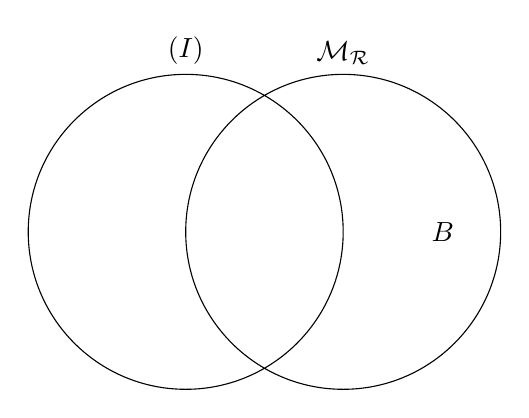
\begin{tikzpicture}
          \draw (-1, 0 ) circle (2)
                (-1, 2 ) node [above] {$\LT(I)$}
                ( 1, 0 ) circle (2)
                ( 1, 2 ) node [above] {$\cal M_R$}
                ( 2, 0 ) node [right] {$B$};
        \end{tikzpicture}
      \end{center}
      
      Either $\LT(f) \in B$ or $\LT(f) \in \LT(I)$.
      In the first case, suppose $\LT(f) = b \in B$.
      Then $f - b \in R - X$ has a smaller leading term than $f$,
      contradicting our choice of $f$.
      Otherwise, suppose $\LT(f) = m \in \LT(I)$.
      Then we can subtract from $f$ any monic polynomial in $I$ with the same leading term,
      again yielding a smaller polynomial in $R - X$.
  \end{description}
\end{proof}

\begin{theorem}
  \label{thm_groebner_basis_product}
  Let $I$ and $J$ be ideals of $R = K[x_1, \ldots, x_n]$, generated by Gr\"obner bases, say
  \begin{align*}
    I &= \pid{f_1, \ldots, f_m} \\
    J &= \pid{g_1, \ldots, g_n}.
  \end{align*}
  Then
  \[ \{ f_ig_j ~|~ 1 \leq i \leq m, 1 \leq j \leq n \} \]
  is a Gr\"obner basis for the ideal product $IJ$.
\end{theorem}
\begin{proof}
  \begin{align*}
    \LT(IJ)
      &= \pid{ \LT(h) ~|~ h \in IJ } \\
      &= \pid{ \LT(fg) ~|~ f \in I, g \in J } \\
      &= \pid{ \LT(f)\LT(g) ~|~ f \in I, g \in J } \\
      &= \pid{ \LT(f) ~|~ f \in I } \pid{ \LT(g) ~|~ g \in J } \\
      &= \LT(I) \LT(J) \\
      &= \pid{ \LT(f_i) ~|~ 1 \leq i \leq m } \pid{ \LT(g_j) ~|~ 1 \leq j \leq n } \\
      &= \pid{ \LT(f_i) \LT(g_j) ~|~ 1 \leq i \leq m, 1 \leq j \leq n } \\
      &= \pid{ \LT(f_i g_j) ~|~ 1 \leq i \leq m, 1 \leq j \leq n }
  \end{align*}
\end{proof}

\begin{theorem}
  \label{thm_groebner_basis_remainder}
  Let $I$ be an ideal of $R$, generated by the Gr\"obner basis $G = \{ g_1, \ldots, g_m \}$. Then
  \begin{enumerate}[label=(\roman*)]
    \item
    Every polynomial $f \in R$ can be written uniquely in the form
    \begin{equation*}
      f = g + r
    \end{equation*}
    where $g \in I$, $r \in R$, and no non-zero term in $r$ is divisible by the leading term of any $g_i$.
    
    \item
    For any polynomial $f \in R$, we have that $f \in I$ if and only if $r = 0$.
  \end{enumerate}
\end{theorem}
\begin{proof}
  \begin{enumerate}[label=(\roman*)]
    \item
    The GPLD algorithm gives $g$ and $r$ satisfying these criteria, demonstrating existence.
    We need only show that these are unique.
    It suffices to show that $r$ is unique, since this uniquely determines $g = f - r$.
    
    Suppose $f = g + r = g' + r'$, with $g, g' \in I$, $r, r' \in R$, and between the non-zero terms of $r$ and $r'$,
    none are divisible by the leading term of any $g_i \in G$.
    Then $r - r' = g' - g \in I$.
    Hence $\LT(r - r') \in \LT(I)$.
    This implies that $\LT(r - r')$ is divisible by some $\LT(g_i)$,
    but this would contradict the fact that no non-zero term in either of $r$ and $r'$ is divisible by any $\LT(g_i)$,
    unless $\LT(r - r') = 0$, whereupon $r = r'$.
    
    \item
    Let $f = g + r$, where $g \in I$ and no non-zero term of $r$ is divisible by any $\LT(g_i)$.

    ($\implies$)
    Suppose $f \in I$.
    Then we can write $f = f + 0$, and this representation is unique by part (i), hence $r = 0$.

    ($\impliedby$)
    Suppose $r = 0$.
    Then $g = g + r = f \in I$.
  \end{enumerate}
\end{proof}

It is an obvious fact that, given any polynomial $f \in K[x_1, \ldots, x_n]$,
we can separate $f$ into its homogeneous components.
That is, we can write
\[ f = \sum_{i = 0}^n f_i^* \]
where $n$ is the total degree of $f$ and $f_i^*$ is homogeneous of degree $i$.

Given a point $P = (a_1, \ldots, a_n) \in \bb A_K^n$, we can even write $f$ in the same form,
but where $f_i^*$ is homogeneous in the variables $(x_1 - a_1), \ldots, (x_n - a_n)$.
E.g., in $\bb Q[x,y]$, given the point $P = (1,1)$, 
\[ x^2 + y^2 = [(x - 1)^2 + (y - 1)^2] + [2(x + 1) + 2(y + 1)] + [2]. \]
This is just the multivariate Taylor series expansion of the polynomial around the point $P$.
This generalizes to the following.

\begin{theorem}
  Let $R = K[x_1, \ldots, x_n]$ and let $I$ be an ideal of $R$ given by a Gr\"obner basis $I = \pid{g_1, \ldots, g_m}$.
  Then $f$ can be written uniquely in the form
  \[ f = \sum_{i=0}^t f_i^*, \]
  where $t = \max\{n \in \bb N ~|~ f \in I^n\}$, $f_i^* \in I^i - I^{i+1}$, and $f_i^* \not\in \LT(I^{i+1})$.
\end{theorem}
\begin{proof}
  By Theorem \ref{thm_groebner_basis_product}, our Gr\"obner basis for $I$ gives us a basis for $I^t$.
  Theorem \ref{thm_groebner_basis_remainder} then applies, allowing us to write
  \[ f = f^*_t + r_t \]
  with $f^*_t \in I^t - I^{t+1}$ and $r_t \in R$, $r_t \not\in \LT(I^t)$.
  Applying Theorems \ref{thm_groebner_basis_product} and \ref{thm_groebner_basis_remainder} $t-1$ more times gives the result.
\end{proof}

Essentially, given finitely polynomials $\{ g_i \}$ forming a Gr\"obner basis for an ideal,
we can uniquely perform a homogenous decomposition of any polynomial $f$ with respect to the $g_i$'s.

This also allows us to show that (over a field of sufficiently large characteristic)
$f \in I^2$ if and only if $f$ and its differential $df$ vanish modulo $I$.
